\documentclass{InsightArticle}

\usepackage[dvips]{graphicx}
\usepackage{float}
\usepackage{subfigure}

\usepackage[dvips,
bookmarks,
bookmarksopen,
backref,
colorlinks,linkcolor={blue},citecolor={blue},urlcolor={blue},
]{hyperref}

\title{Smart Nearest Neighbors}

% 
% NOTE: This is the last number of the "handle" URL that 
% The Insight Journal assigns to your paper as part of the
% submission process. Please replace the number "1338" with
% the actual handle number that you get assigned.
%
\newcommand{\IJhandlerIDnumber}{3250}

% Increment the release number whenever significant changes are made.
% The author and/or editor can define 'significant' however they like.
\release{0.00}

% At minimum, give your name and an email address.  You can include a
% snail-mail address if you like.

\author{David Doria}
\authoraddress{Army Research Laboratory, Aberdeen MD}


\begin{document}

\IJhandlefooter{\IJhandlerIDnumber}


\ifpdf
\else
   %
   % Commands for including Graphics when using latex
   % 
   \DeclareGraphicsExtensions{.eps,.jpg,.gif,.tiff,.bmp,.png}
   \DeclareGraphicsRule{.jpg}{eps}{.jpg.bb}{`convert #1 eps:-}
   \DeclareGraphicsRule{.gif}{eps}{.gif.bb}{`convert #1 eps:-}
   \DeclareGraphicsRule{.tiff}{eps}{.tiff.bb}{`convert #1 eps:-}
   \DeclareGraphicsRule{.bmp}{eps}{.bmp.bb}{`convert #1 eps:-}
   \DeclareGraphicsRule{.png}{eps}{.png.bb}{`convert #1 eps:-}
\fi


\maketitle


\ifhtml
\chapter*{Front Matter\label{front}}
\fi

\begin{abstract}
\noindent

This document presents an implementation of two algorithms, Voronoi Neighbors and BSP Neighbors, to find nearest neighbors of a point in a point set that are more intelligent than a ``K nearest neighbors'' or a ``all neighbors within a radius'' query. This type of nearest neighbor query is more computationally expensive, but typically returns a ``better'' set of neighbors. The BSP Neighbors search ensures that there is less local duplication, while the Voronoi Neighbors search ensures that the spatial arrangement of the neighbors is as uniform as possible.

These algorithms are explained in "Point Primitives for Interactive Modeling and Processing of 3D Geometry".

The code is available here:
https://github.com/daviddoria/SmartNearestNeighbors

\end{abstract}

\IJhandlenote{\IJhandlerIDnumber}

\tableofcontents
%%%%%%%%%%%%%%%%%%%%
\section{Introduction}
This document presents an implementation of an algorithm to perform a morphological opening on a graph. This opening consists of a series of erosions, followed by a series of dilations. This is often done as a first step in contour closure algorithms.

These implementations are based on the algorithms described in \cite{Pauly2003}.

%%%%%%%%%%%%%%%%%%%%
\section{Voronoi Neighbors}
Voronoi cell V_i of q_i is
V_i = {x in ||x-q_i|| <= ||x-q_j|| all j in kNeighbors, j!=i}
Voronoi neighbors are a subset of the kNeighbors whose Voronoi cell is adjacent to V_p, 
the Voronoi cell of the point for which the kNeighbors were found

%%%%%%%%%%%%%%%%%%%%
\section{BSP Neighbors}
The morphological dilation operation on a graph is only defined on a graph which has previously been eroded. The dilation adds back edges to current end points that were removed in a previous erosion operation.

Each nearest neighbor point defines a halfspace. The BSP neighbors are a subset of the KNearestNeighbors
which are in the intersection of all of the halfspaces induced by the kNearestNeighbor points.
  
Each kNeighbor defines a halfspace as:
(x-q_i).(p-q_i) >= 0
x is a test point (the collection of x that fit this criterion is exacly the halfspace)
q_i is the ith nearest neighbor point
p is the center point (for which the kNearest points were found)

% \begin{figure}[H]
% \centering
% \subfigure[A brown rectangular object.]
%   {
%   \includegraphics[width=0.3\linewidth]{images/rectangleSolid}
%   \label{fig:EdgeImage:Image}
%   }
% \subfigure[A simple edge pixel classification. White pixels are edge pixels.]
%   {
%   \includegraphics[width=0.3\linewidth]{images/rectangleSolidEdgeThresholded}
%   \label{fig:EdgeImage:EdgeImage}
%   }
% \caption{An image of an object and its corresponding edge image.}
% \label{fig:EdgeImage}
% \end{figure}

% \begin{figure}[H]
%   \centering
%   \includegraphics[width=0.3\linewidth]{images/rectanglePoints}
%   \caption{A solid point cloud of a rectangular 2D object.}
%   \label{fig:SolidPointCloud}
% \end{figure}

%%%%%%%%%%%%%%%%%%%%
\section{Demonstration}
\label{sec:Demonstration}
In this Figure \ref{fig:1Iteration}, we show the result of one erosion and one dilation.
\begin{figure}[H]
\centering
\subfigure[Original graph.]
  {
  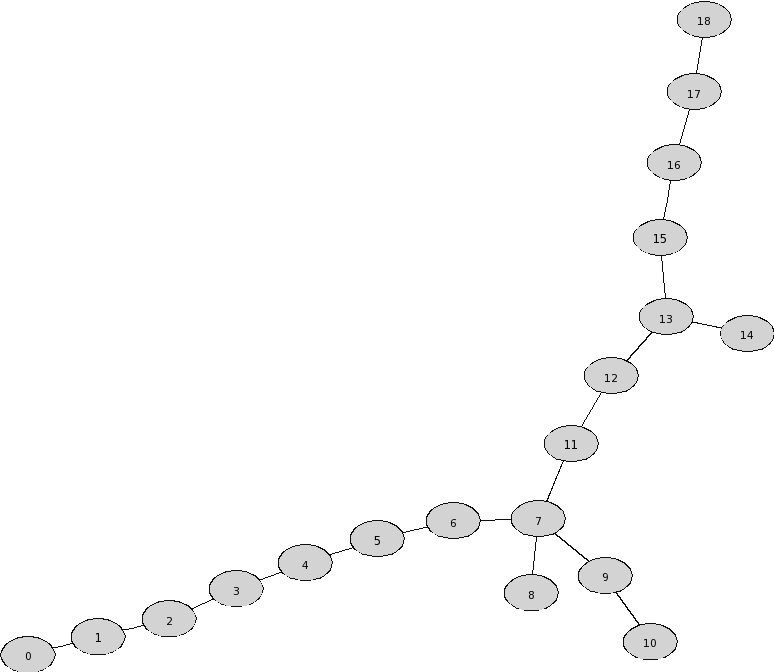
\includegraphics[width=0.3\linewidth]{images/opening1_0}
  \label{fig:1Iteration:Original}
  }
\subfigure[Graph after 1 erosion.]
  {
  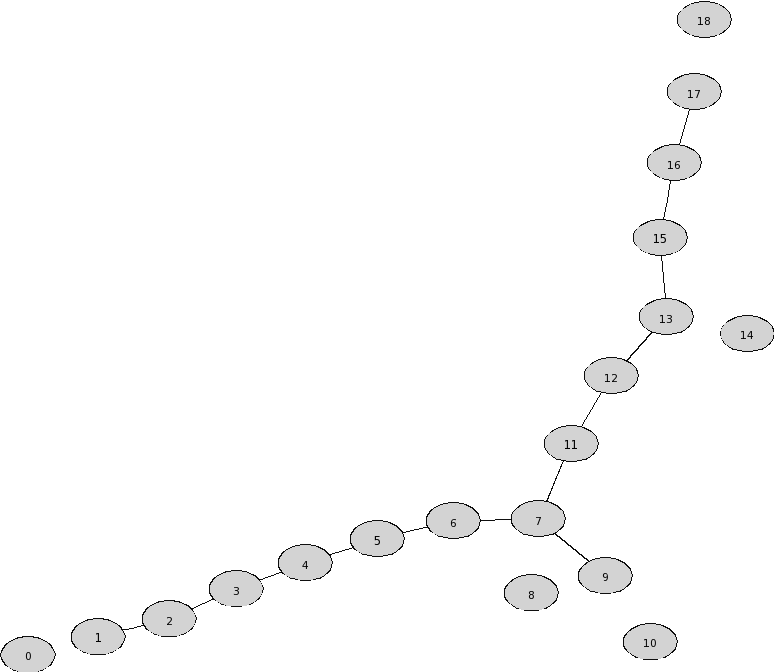
\includegraphics[width=0.3\linewidth]{images/opening1_1}
  \label{fig:1Iteration:1Erosion}
  }
\subfigure[Graph after 1 erosion and 1 dilation.]
  {
  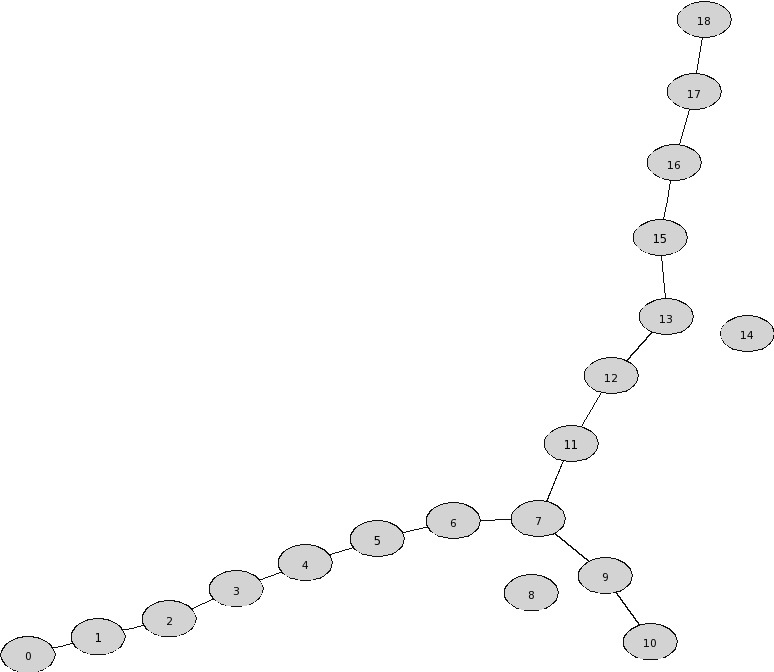
\includegraphics[width=0.3\linewidth]{images/opening1_2}
  \label{fig:1Iteration:1Erosion1Dilation}
  }
\caption{Erosions = 1, Dilations = 1}
\label{fig:1Iteration}
\end{figure}

In this Figure \ref{fig:1Iteration}, we show the result of one erosion and one dilation.
\begin{figure}[H]
\centering
\subfigure[Original graph.]
  {
  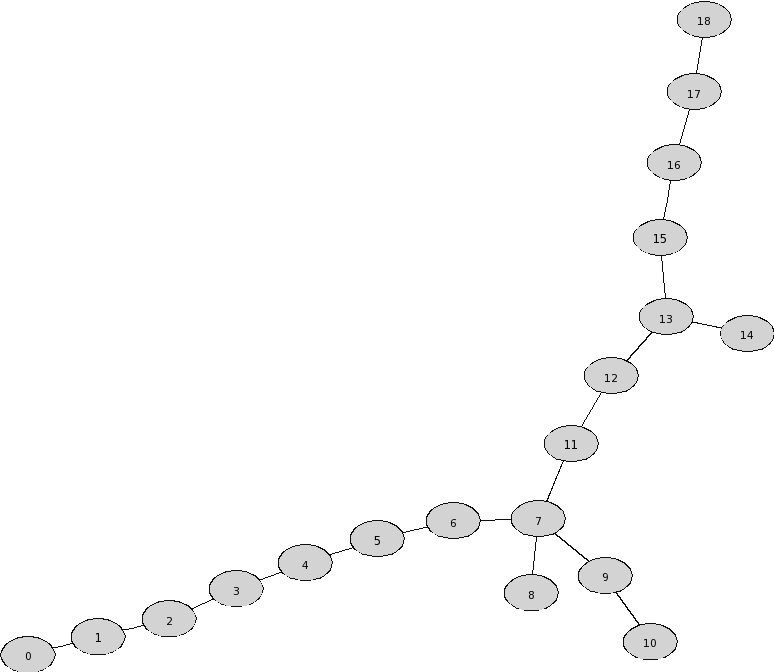
\includegraphics[width=0.19\linewidth]{images/opening0}
  \label{fig:2Iterations:Original}
  }
\subfigure[Graph after 1 erosion.]
  {
  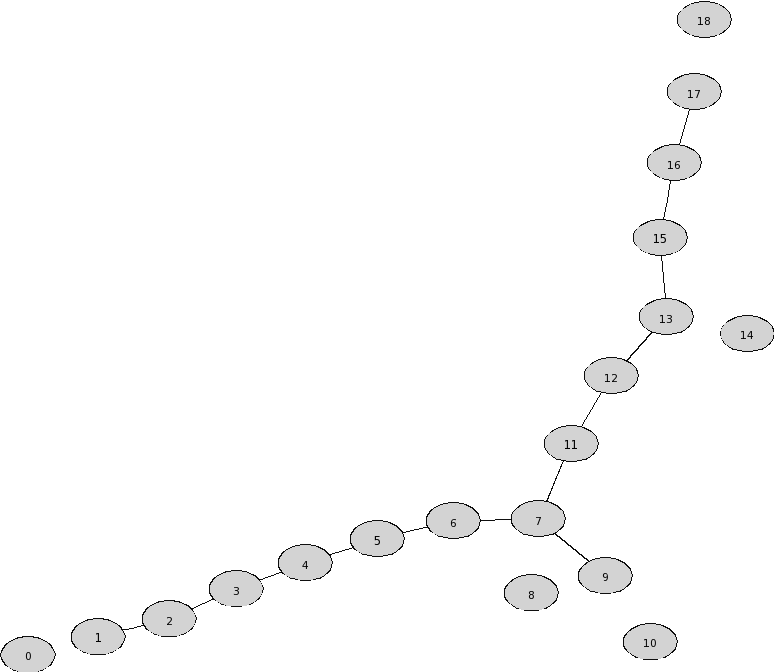
\includegraphics[width=0.19\linewidth]{images/opening1}
  \label{fig:2Iterations:1Erosion}
  }
\subfigure[Graph after 2 erosions.]
  {
  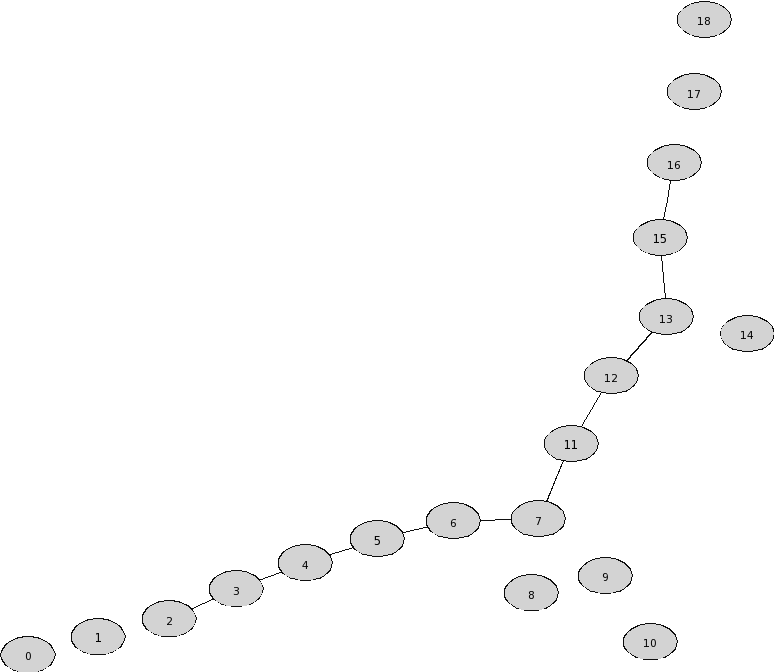
\includegraphics[width=0.19\linewidth]{images/opening2}
  \label{fig:2Iterations:2Erosions}
  }
\subfigure[Graph after 2 erosions and 1 dilation.]
  {
  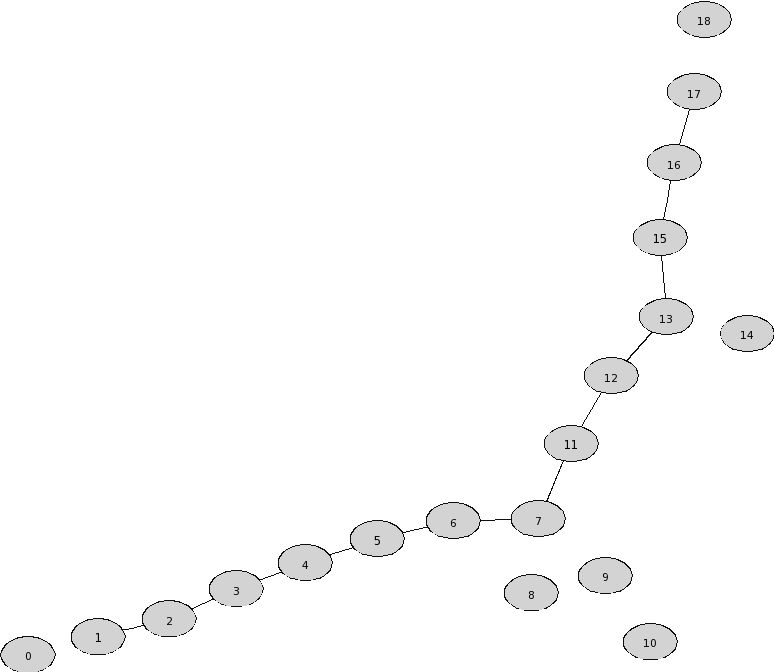
\includegraphics[width=0.19\linewidth]{images/opening3}
  \label{fig:2Iterations:2Erosions1Dilation}
  }
\subfigure[Graph after 2 erosions and 2 dilations.]
  {
  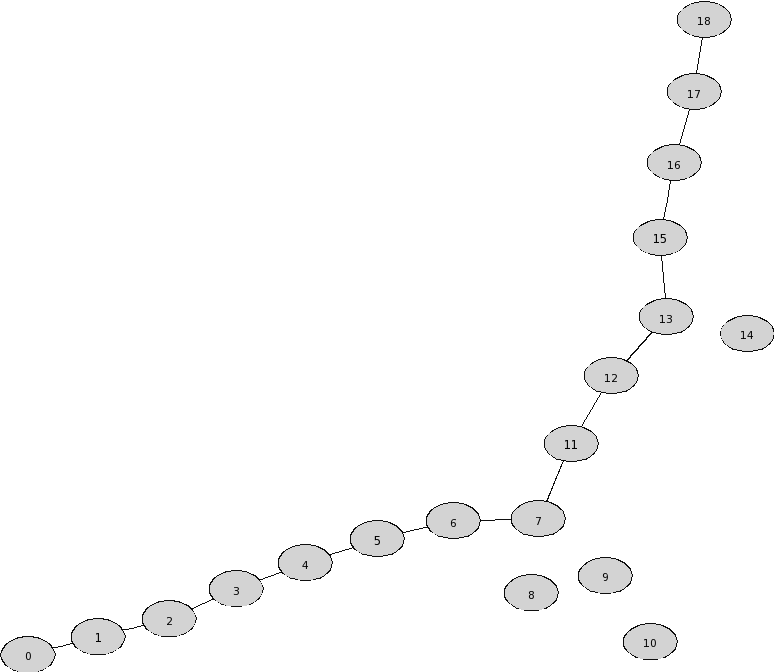
\includegraphics[width=0.19\linewidth]{images/opening4}
  \label{fig:2Iterations:2Erosions2Dilations}
  }
\caption{Erosions = 2, Dilations = 2}
\label{fig:2Iterations}
\end{figure}

%%%%%%%%%%%%%%%
\section{Code Snippet}

\begin{verbatim}

\end{verbatim}

\bibliography{InsightJournal}

\end{document}